% !Tex root = Vorlage.tex
\newpage
\section{Grundlagen zum Begriff}
Im folgenden Abschnitt sollen die Grundlagen für eine weitere Auseinandersetzung mit den Folgen von Unconscious Bias geschaffen werden. Dabei wird der Begriff des Bias diskutiert, dessen evolutionäre Vorgeschichte umrissen und Arten des Bias kategorisiert sowie besprochen.\\

\subsection{Begriffsdiskussion}
Der englische Begriff des \glqq Bias\grqq~lässt sich im Deutschen als \glqq Vorurteil\grqq~oder \glqq Voreingenommenheit\grqq~übersetzen. Da die Fachdiskussion vor allem im englischsprachigen Raum vorangetrieben wird, wollen wir in diesem Beitrag auch den Begriff des \glqq Bias\grqq~verwenden. Motiviert ist dies dadurch, dass obengenannte Übersetzung nämlich - wie in den folgenden Abschnitten herausgearbeitet werden soll - nicht einfach übersetzt werden kann und durch den wissenschaftlichen Diskurs bereits viel breiter besetzt ist, als der Begriff \glqq Vorurteil\grqq~es vermuten lässt. \\

Die offizielle Beratungsstelle der Europäischen Union wendet den Begriff der \glqq Wahrnehmungsverzerrung\grqq\footnote{http://www.anti-bias.eu/unconsciousbias/definition/} an, der bereits deutlich themenbezogener scheint. Die Verzerrung der Wahrnehmung kann dabei bewusst in Form eines \glqq Conscious Bias\grqq~oder unbewusst als \glqq Unconscious Bias\grqq~stattfinden.

\begin{figure}[htbp]
    \subfigure[Schrittweise Vergrößerung der Gruppe.]
    {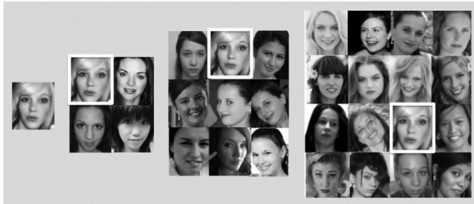
\includegraphics[width=0.49\textwidth]{Bilder/cheerleader-effekt-1.jpg}}
    \subfigure[Auswirkung der Vergrößerung der Gruppe auf die Wahrnehmung von Attraktivität.]
    {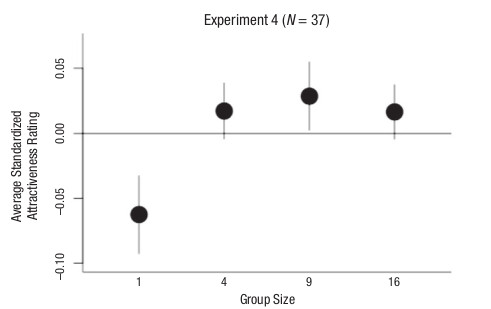
\includegraphics[width=0.49\textwidth]{Bilder/cheerleader-effekt-2.jpg}}
\caption{Der Cheerleader-Effekt als einfaches Beispiel für einen Unconscious Bias.}
\label{fig:beispiel-unconscious-bias}
\end{figure}

\subsection{Kategorisierung des Bias}
Bias wird auf unterschiedlichen kognitiven Ebenen wahrgenommen, meist über komplexe Abläufe zwischen visuellen Ebenen. Um ein Gefühl dafür zu geben, was ein Bias ist, soll nun ein simpler, hauptsächlich visueller Bias als Beispiel angeführt werden: der Cheerleader-Effekt. Dazu sind Grafiken aus dem Paper von Walker und Vul \cite{WAL14} in Abbildung \ref{fig:beispiel-unconscious-bias} aufgeführt. \\

Die Forscher fassen den Cheerleader-Effekt so zusammen (frei aus dem Englischen übersetzt):
\begin{enumerate}
	\item Das visuelle System verarbeitet automatisch ein Ensemble der Gesichter, die in der Gruppe präsentiert werden.
	\item Individuelle Mitglieder der Gruppe werden voreingenommen(\glqq biased\grqq) wahrgenommen mit Tendenz hin zum Durchschnittswert der Attraktivität des Ensembles.
	\item Durchschnittliche Gesichter wirken attraktiv.
\end{enumerate}

Dieser Befund steht im Konflikt zu unseren Alltagserfahrungen. Im Alltag haben wir den Eindruck, unsere Entscheidungen selbst zu treffen aufgrund rationaler Befunde. Wir nehmen die Realität wahr, ordnen sie ein und treffen unsere Entscheidung, in diesem Fall bezüglich der Schönheit eines anderen Menschen. Die Studie von Walker und Vul legt nun nahe, dass dieses Verfahren fehlerhaft ist: Zwar bewerten wir die Attraktivität einer anderen Person selbst, aber die Daten, auf die wir dabei zurückgreifen, sind korrumpiert. Bewerten wir die Attraktivität einer Person außerhalb einer Gruppe, so schätzen wir sie weniger attraktiv ein, als wenn sie Teil einer Gruppe wäre. \\

\begin{figure}[htbp]
	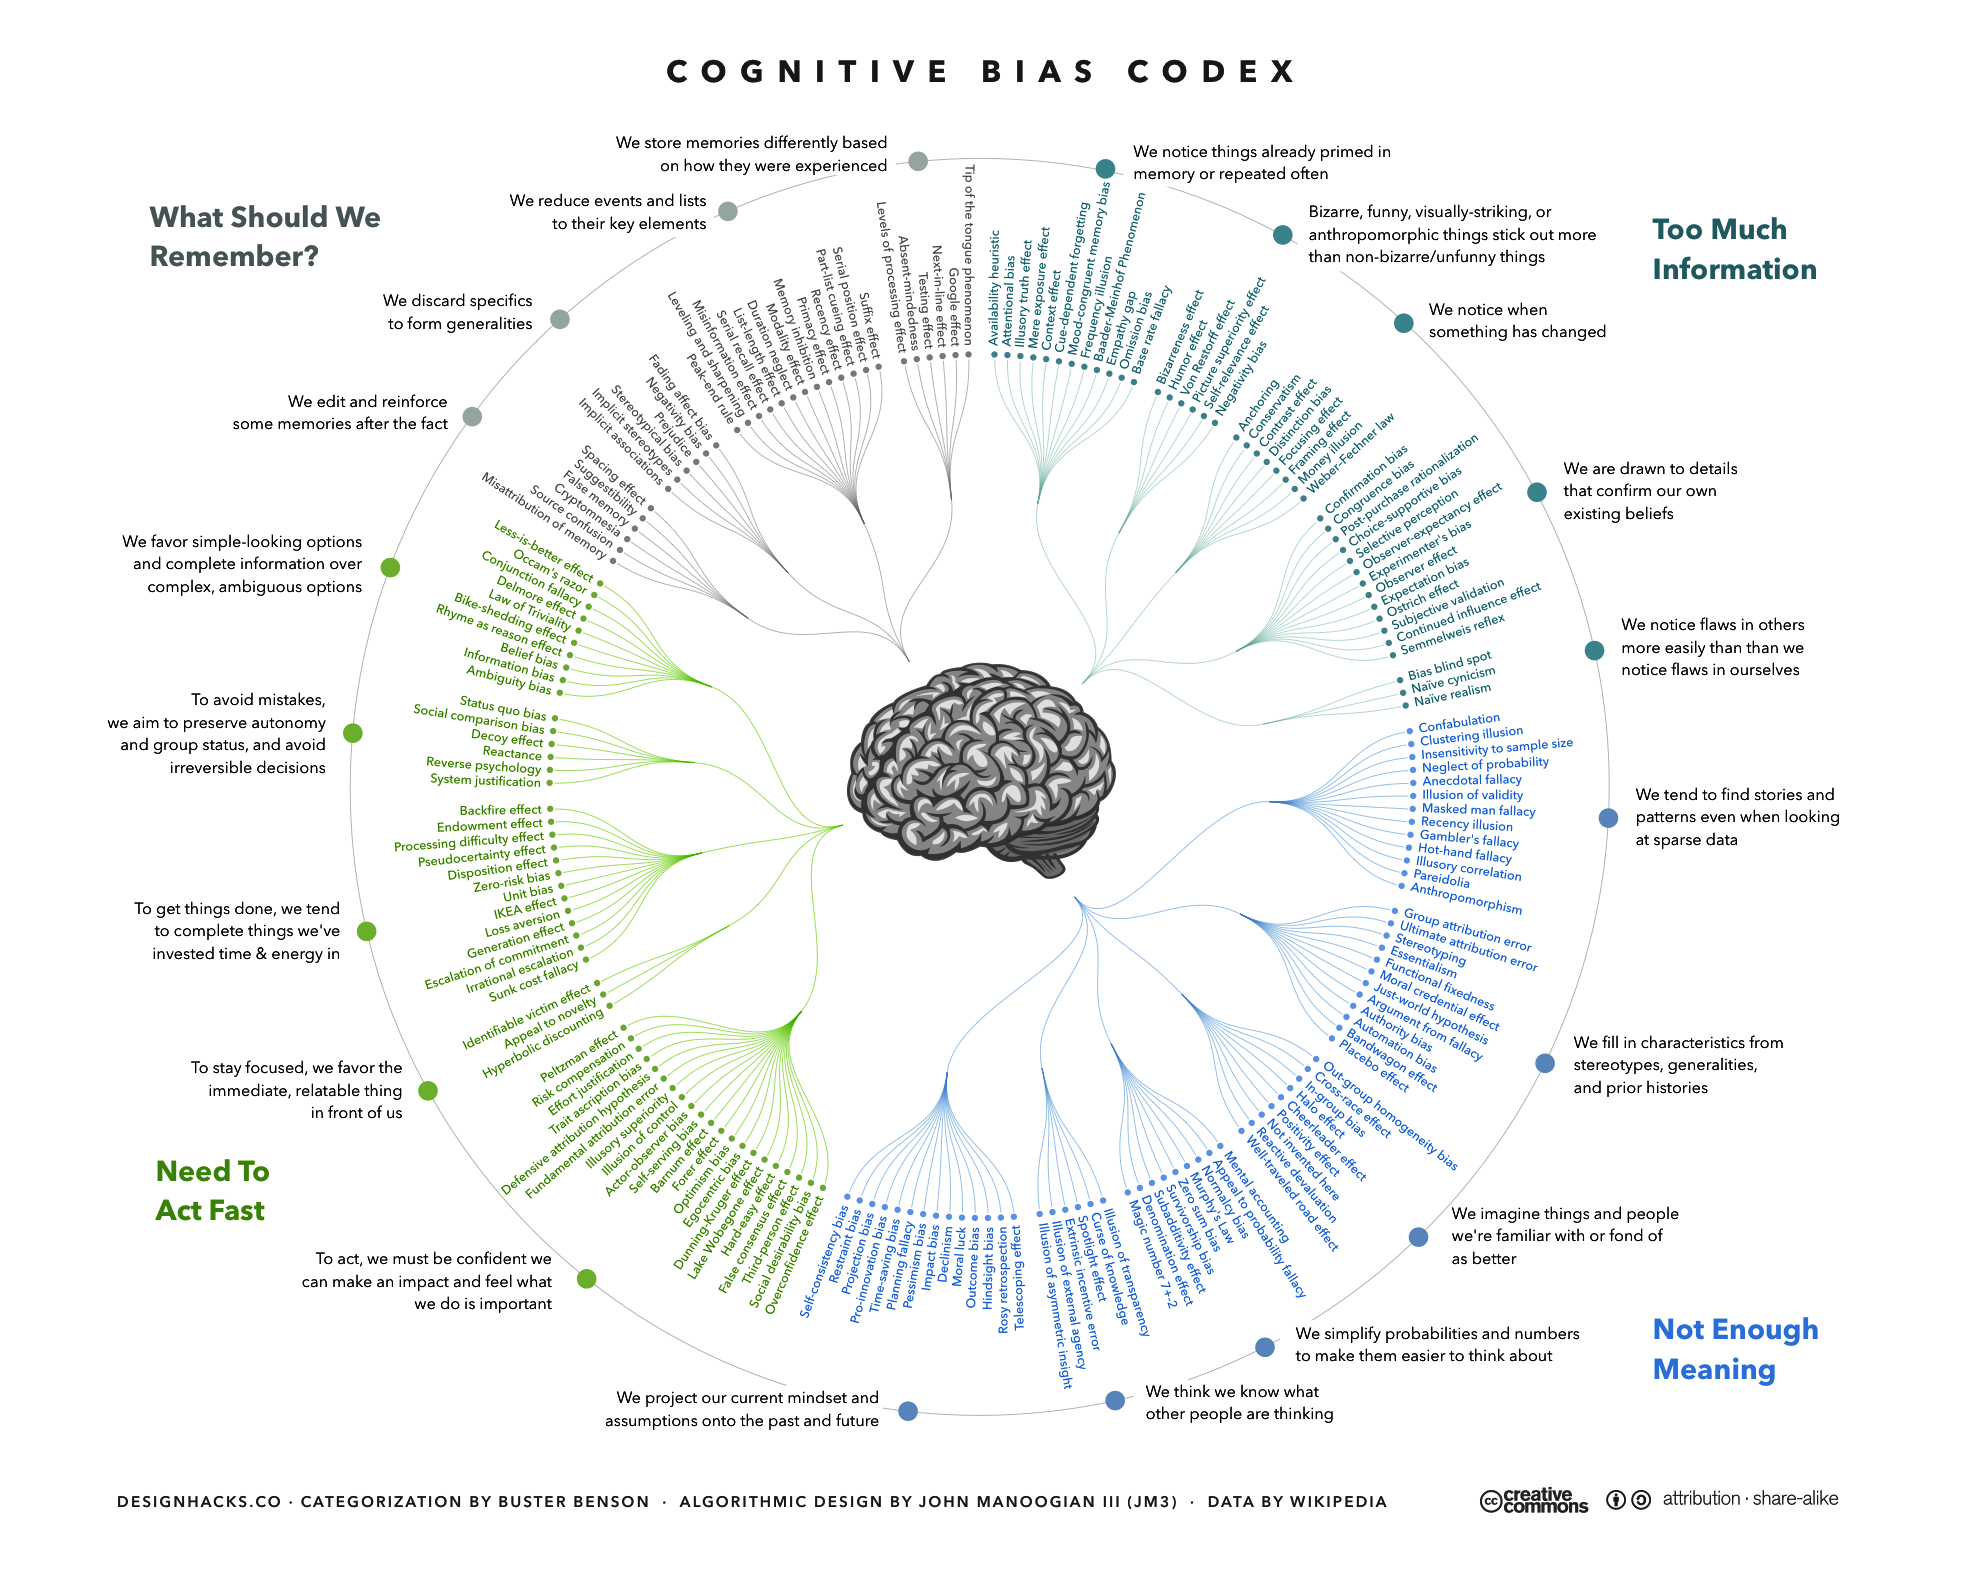
\includegraphics[width=0.95\textwidth]{Bilder/cognitive-bias-codex.png}
	\caption{Übersicht aller in der Wikipedia aufgeführten Cognitive Biases. Grafik von \href{https://commons.wikimedia.org/w/index.php?curid=57942404}{John Manoogian III.}, CC BY-SA 4.0.}
\label{fig:cognitive-bias-codex}
\end{figure}

Unsere Wahrnehmung der Realität ist verzerrt - wir urteilen auf Basis der unwahren Annahme, dass wir Menschen in Gruppen ebenso wahrnehmen wie Menschen außerhalb von Gruppen. All das geschieht unbewusst - ein Unconscious Bias also. Dabei ist der Cheerleader-Effekt ein harmloser Unconscious Bias. Im schlimmsten Fall gehen wir vielleicht mit einer Person aus, die wir für attraktiver halten, als sie es eigentlich ist. Das schadet vielleicht unserem Ego, bleibt aber für uns und die Person folgenfrei. \\

Der Cheerleader-Effekt ist bei Weitem nicht der einzige Bias, der unsere Wahrnehmung beeinflusst und unsere Urteilsfindung trügt. Die Wikipedia führt eine erstaunliche Liste von über 170 Cognitive Biases auf.\footnote{\url{https://en.wikipedia.org/wiki/List_of_cognitive_biases}} Der Blogger John Manoogian III. hat eine Grafik (Abb. \ref{fig:cognitive-bias-codex}) erstellt, die eine Übersicht über alle bekannten Biases verschafft. Sie bezieht sich auf einen Artikel des Autoren Buster Benson,\footnote{Auf dessen Blog \href{https://betterhumans.coach.me/cognitive-bias-cheat-sheet-55a472476b18}{betterhumans.coach.me} abzurufen} der sich mit dem Thema Bias eingehend auseinandersetzt. \\

Benson schlägt eine Kategorisierung von Bias in vier Gruppen vor. Diese Gruppen führt er auf die Ursachen der Entstehung der in ihnen enthaltenen Biases zurück. Diesem Schema folgend soll im folgenden Abschnitt eine Übersicht über bekannte Biases gegeben werden. Zu jeder Kategorie wird ein Bias ausführlich vorgestellt und seine Auswirkungen auf Führungsentscheidungen besprochen.

\subsubsection{Zu viele Informationen}
In der modernen Welt werden wir mit Informationen überflutet. Unser Gehirn filtert rigoros nahezu alle Informationen aus und reduziert auf ein bearbeitbares Minimum an eingehenden Informationen. Dabei können folgende Muster erkannt werden:
\begin{itemize}
	\item Wir bemerken Dinge besondert stark, mit denen wir bereits Assoziationen gebildet haben und die bereits in unserem Gedächtnis gespeichert sind.\cite{HAS77}
	\item Wir erinnern uns besonders gut an ungewöhnliche und überraschende Erlebnisse.\cite{BAU01}
	\item Wir können relative Werte wesentlich besser einschätzen als absolute Werte. \cite{KAH06}
	\item Wir werden zu Dingen hingezogen, die unsere bisherigen Empfindungen bestätigen.\cite{PLO93}
	\item Wir sehen Fehler in Anderen einfacher als in uns selbst.\cite{PRO02}
\end{itemize}

Der \glqq Mere-Exposure-Effekt\grqq, zu Deutsch \glqq Effekt des bloßen Kontakts\grqq, ist ein in der wissenschaftlichen Literatur seit den 60er Jahren breit diskutierter Unconscious Bias. Entdeckt 1968 von Robert Zajonc\cite{ZAJ68} erklärt der Mere-Exposure-Effekt maßgeblich, wie wir Gewohnheiten und Präferenzen entwickeln. Zajonc fand heraus, dass unsere Meinung von einer Sache oder einer Person stark damit korreliert, wie oft wir Kontakt mit ihr haben. Je häufiger wir das Logo einer Marke sehen, desto besser denken wir über die Marke. Die Crux: Dieser Kontakt kann unbewusst stattfinden und hat doch den selben Effekt wie das bewusste Wahrnehmen des Kontakts. \\

Sehr plastisch gezeigt hat den Mere-Exposure-Effekt Patricia Pliner von der University of Toronto. In ihrem Artikel \glqq The Effect of Mere Exposure on Liking for Edible Substances\grqq\cite{PLI82} präsentiert sie die Ergebnisse einer Untersuchung an männlichen Bachelorstudenten. Den Versuchspersonen gab sie 35 unbekannte Fruchtsaftproben zum Probieren. Was die Versuchsteilnehmer nicht wussten: Ihnen wurden nur drei unterschiedliche Säfte vorgesetzt. Ein Saft war 20 Mal vertreten, ein Zweiter zehn Mal und ein Dritter fünf Mal. Zusätzlich wurde ein vierter Saft gar nicht zum Probieren angeboten. Zur Unkenntlichmachung wurde den Säften eine zufällige Dosis Lebensmittelfarbe zugefügt. \\

 \begin{figure}[htbp]
	\begin{center}
		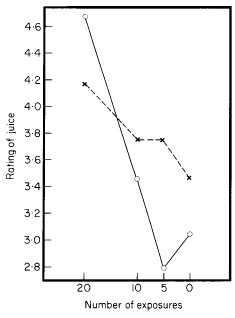
\includegraphics[width=0.3\textwidth]{Bilder/exposure-effekt.jpg}
		\caption{Die Abbildung zeigt die durchschnittliche Präferenz der 24 Probanden für einen Fruchtsaft in Abhängigkeit der Anzahl an Kontakten mit dem Saft. Der Graph mit zusammenhängender Linie zeigt die Ergebnisse der ersten Sitzung, der Graph mit der gestrichelten Linie die der zweiten Sitzung.}
		\label{fig:mere-exposure-effekt}
	\end{center}
\end{figure}

Im Anschluss wurde den Probanden je eine Probe der vier Säfte vorgesetzt. Sie wurden gebeten, die Bitterkeit der Säfte zu bewerten, was die erste Sitzung beendete. Das Prozedere wurde in einer zweiten Sitzung wiederholt. Dabei wurde die Anzahl der dargebotenen Säfte vertauscht: Der Saft, der in der ersten Sitzung 20 Mal zum Probieren vertreten war, fehlte nun komplett. Der Saft jedoch, der vorher gar nicht zum Probieren angeboten wurde, war nun 20 Mal dargereicht. Nach der zweiten Verkostung hatten die Versuchsteilnehmer somit jeden Saft 20 Mal probiert. Anschließend bewerteten die Versuchsteilnehmer die Säfte ein zweites Mal. \\

Das Ergebnis der Studie ist in Abbildung \ref{fig:mere-exposure-effekt} zu sehen. Es ist klar zu erkennen, dass die Säfte positiver bewertet wurden, je häufiger sie getrunken wurden. Das gilt auch für das Ergebnis der zweiten Sitzung, hier fällt der Mere-Exposure-Effekt aber weniger stark aus. Dies liegt daran, dass die Teilnehmer zu diesem Zeitpuntk jeden Saft 20 Mal verkostet hatten und sich somit ein Gedächtnis der Präferenz gebildet hat. \\

Für Führungskräfte hat der Mere-Exposure-Effekt als Folge, dass sie ihre eigenen Präferenzen kritisch hinterfragen sollten. Sie sollten regelmäßig bewerten, aus welchen Gründen sie Entscheidungen treffen. Dabei ist explizit zu beachten, dass persönliche Präferenz durch den Mere-Exposure-Effekt beeinflusst sein kann. Man läuft Gefahrt, Optionen nicht zu beachten, die in der Situation besser angebracht wären. \\

Auch bei Personalentscheidungen muss der Mere-Exposure-Effekt berücksichtigt werden. Führungskräfte müssen sich fragen, welche Kompetenzen eine Person hat und wie diese zu einer Aufgabe passen. Diese Erwägung ist von persönlicher Präferenz zu trennen, um nicht von Wahrnehmungsverzerrungen wie dem Mere-Exposure-Effekt beeinflusst zu werden. \\

Auf der anderen Seite kann sich eine Führungskraft den Mere-Exposure-Effekt zu Nutze machen. Beispielsweise, wenn sie die Sympathie ihrer Mitarbeiter erlangen möchte. Orientiert sich die Führungskraft in ihrem Verhalten am Transformational Leadership, dann ist es unabdingbar, ein gutes Verhältnis zu den geführten Mitarbeitern aufzubauen. Ein wichtiger Grundstein hierfür ist, und das sagt uns der Mere-Exposure-Effekt, die Präsenz der Führungskraft. Das kann bedeuten, gemeinsam mit den Mitarbeitern ein Büro zu teilen. Aber auch, dass man in einer Videokonferenz darauf achtet, die eigene Webcam einzuschalten, damit man gesehen werden kann. Auch das Wiederholen von Visionen ist nach der Theorie des Mere-Exposure-Effekt zuträglich zu einer positiven Meinung der Mitarbeiter über die wiederholte Vision. 

\subsubsection{Zu wenig Bedeutung}
Im Verhältnis zur gewaltigen Menge an Informationen, mit der unser Gehirn jeden Tag konfrontiert ist, nehmen wir nur einen winzigen Ausschnitt der Realität bewusst wahr. Trotzdem verwenden wir die uns vorhandenen Informationen, extrapolieren sie und versuchen, Sinn oder Bedeutung in den Informationen zu finden. Dabei unterlaufen uns permanent Fehler:
\begin{itemize}
	 \item Wir finden Muster und Sinn selbst bei unzureichender Datenlage. \cite{MUL90}
	 \item Wir füllen Informationslücken mit Allgemeingültigem und Stereotypen. \cite{MIL63}
	 \item Wir stellen uns Dinge und Menschen, mit denen wir vertraut sind, besser vor als solche, die uns unbekannt sind. \cite{TAY81}
	 \item Wir vereinfachen und verfälschen Wahrscheinlichkeiten und Zahlen, abhängig von Situationen. \cite{MEE10}
	 \item Wir meinen zu wissen, was andere denken. \cite{SAV03}
	 \item Wir projizieren unsere jetzigen Bewusstseinszustände und Annahmen in Vergangenheit und Zukunft. \cite{ROE12}
\end{itemize} 

Ein klassisches sozialpsychologisches Beispiel zur Suche nach Bedeutung, wo keine ist, ist das Robbers-Cave-Experiment (Räuberhöhlenexperiment). Das Experiment wurde in den 50er Jahren von Muzafer Sherif durchgeführt.\cite{SHE61} Im Zentrum des Experiments steht Sherifs Theorie des realistischen Gruppenkonflikts. \\

Zwei Gruppen von Jungen im jugendlichen Alter wurden in einem von den Forschern veranstalteten Ferienlager gebildet. Das Experiment wurde im Robbers Cave Nationalpark durchgeführt - daher rührt auch der Name. Eine Karte des Lagers ist in Abbildung \ref{fig:robbers-cave-map} zu sehen.\\

Die beiden Gruppen gaben sich nun Namen - die \glqq Klapperschlangen\grqq~und die \glqq Adler\grqq~- und führten unter Anleitung der Forscher Teambuildingmaßnahmen durch. Nach dieser initialen Phase fügten die Forscher eine kompetitive, zweite Phase an. \\

Die beiden Gruppen traten in unterschiedlichen Szenarien gegeneinander an, bei denen es um die Verteilung von Resourcen ging. Besonders an diesen Wettkämpfen war, dass nur die Gewinner des Konflikts Zugang zu den Ressourcen bekamen - es gab keine Trostpreise für die Gruppe, die verlor.\footnote{Der Ablauf des Experiments wurde der ausführlichen Zusammenfassung von \href{http://livros01.livrosgratis.com.br/ps000162.pdf}{Christopher D. Green der York University, Toronto, Ontario} entnommen (Abgerufen 11.06.2018).} \\ 

 \begin{figure}[htbp]
	\begin{center}
		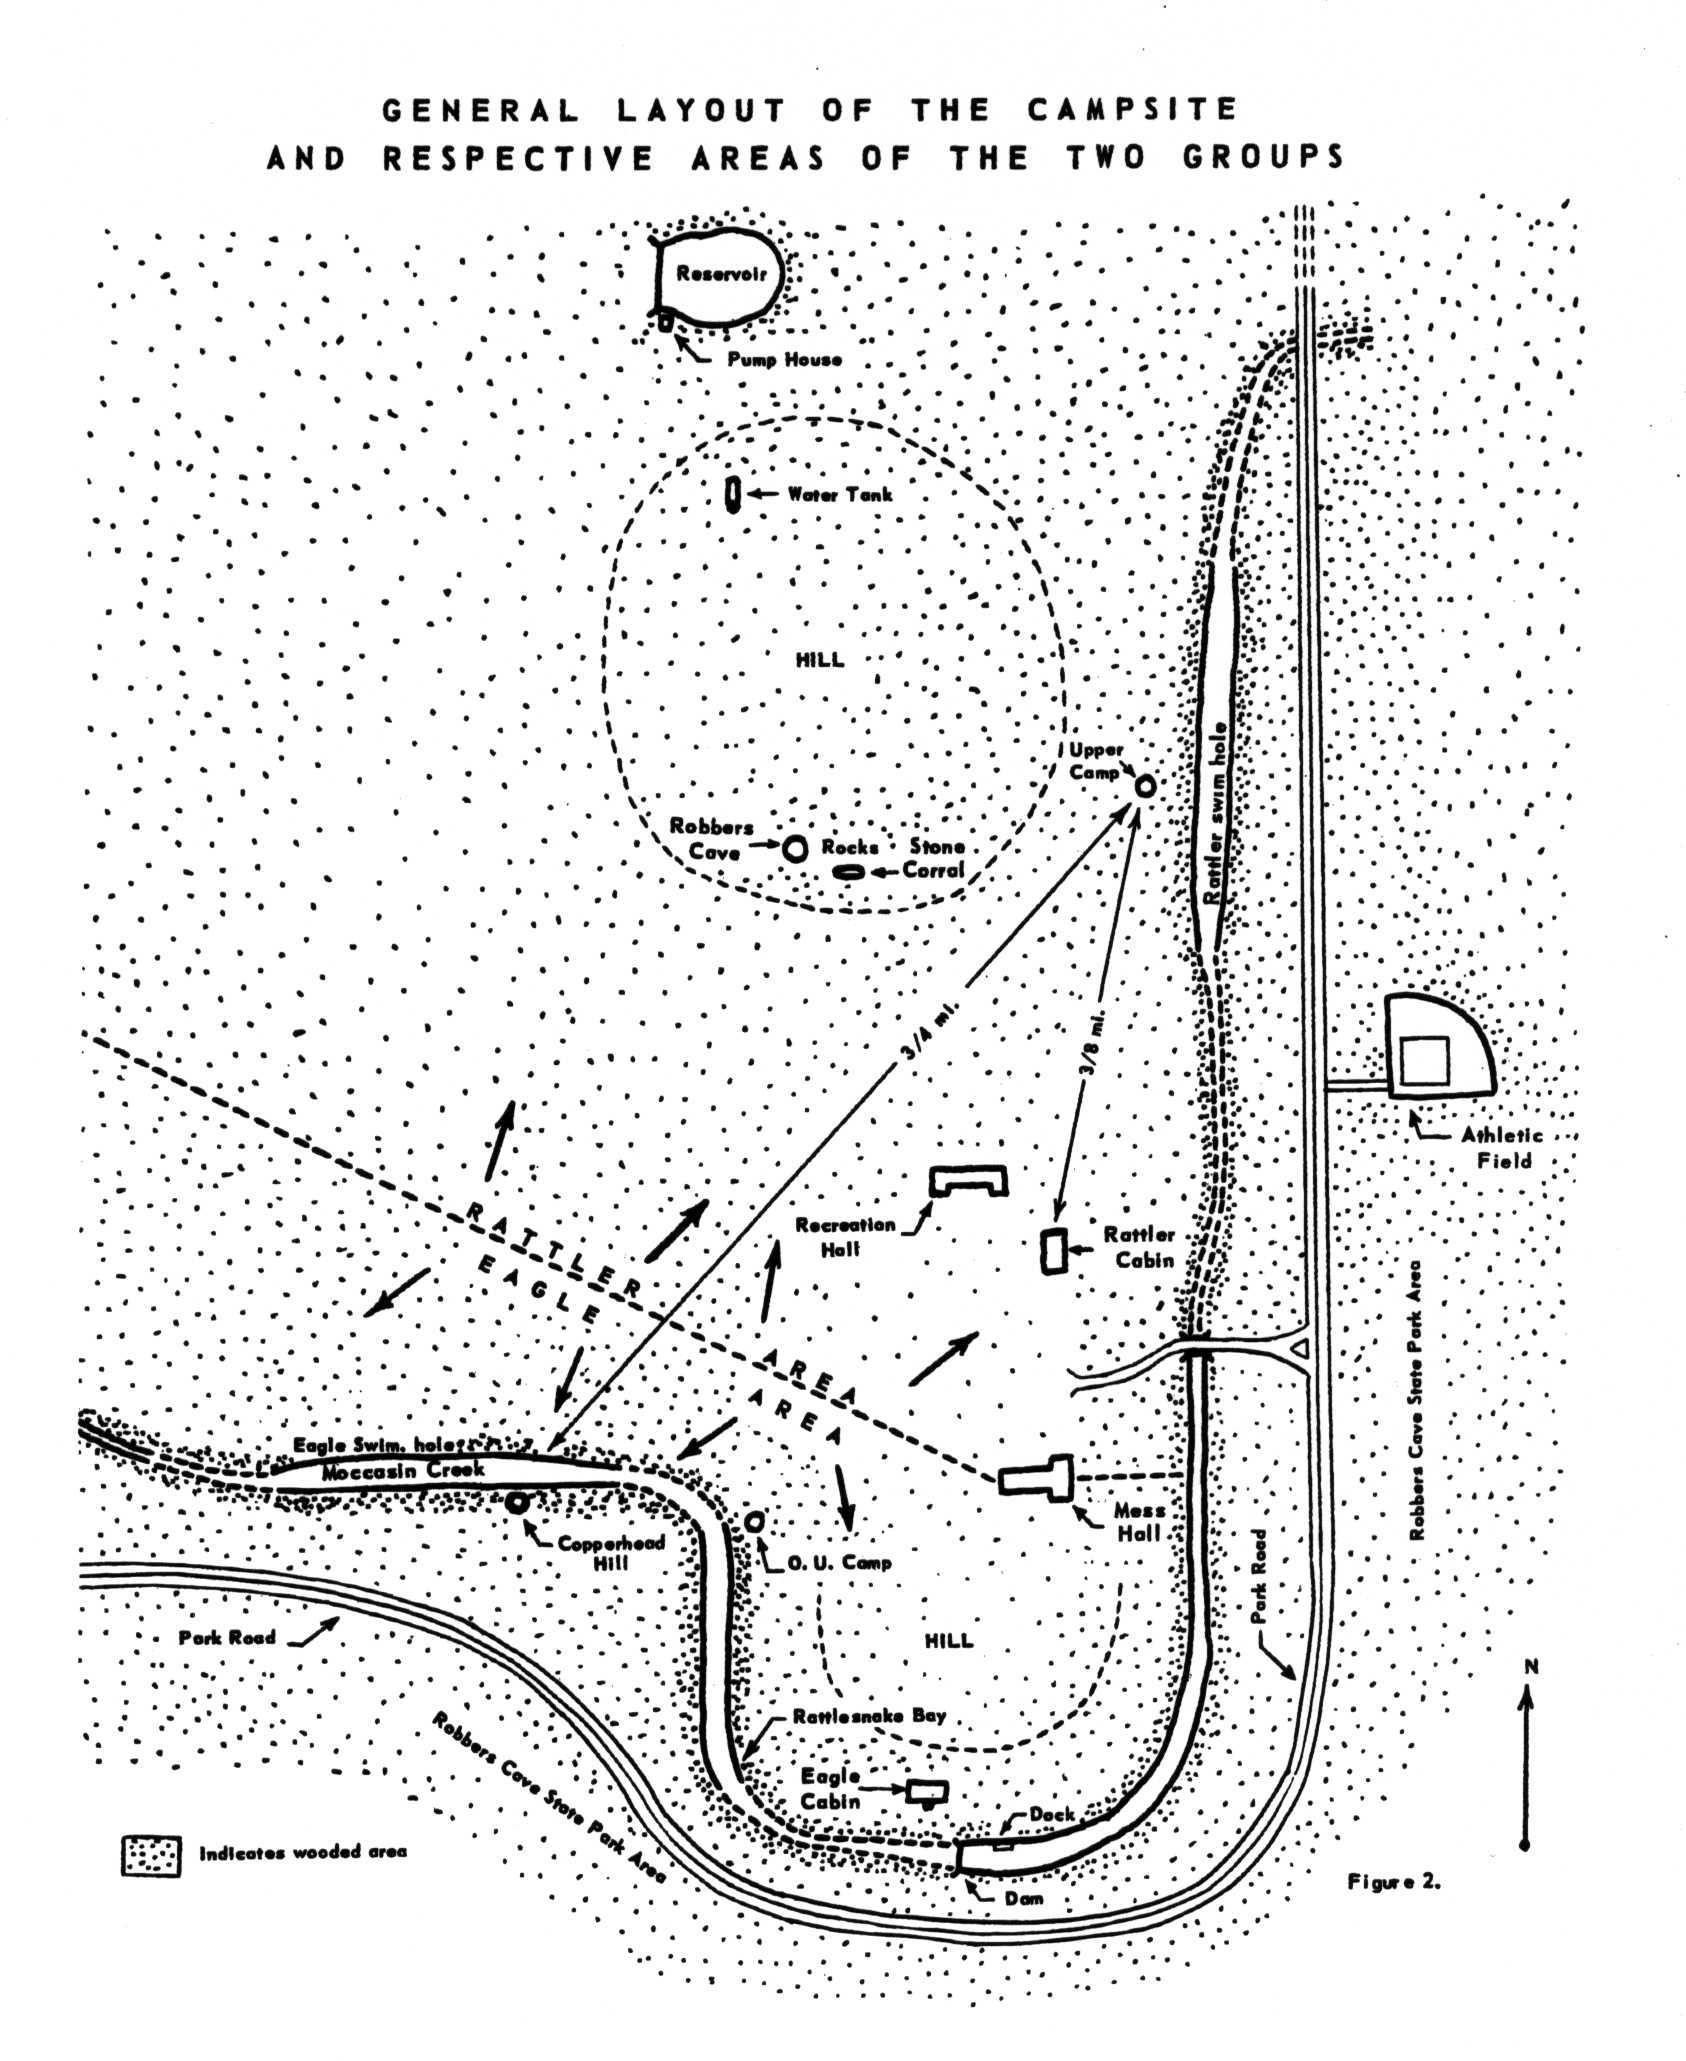
\includegraphics[width=0.5\textwidth]{Bilder/robbers-cave-map.jpg}
		\caption{Die Karte des Ferienlagers, in dem das Robbers-Cave-Experiment durchgeführt wurde.}
		\label{fig:robbers-cave-map}
	\end{center}
\end{figure}

Diese zweite Phase führte zu einem Konflikt zwischen Klapperschlangen und Adlern, der sich zunehmend verschlimmerte. Die Klapperschlangen verbrannten eine verwaiste Flagger der Adler, woraufhin diese zur Hütte der Klapperschlangen zogen und sie verwüsteten (Abbildung \ref{fig:phase-zwei}, rechts). \\

Die Sympathiebewertungen der beiden Gruppen (Abbildung \ref{fig:phase-zwei}, links) spiegelt diese Aggression wider: Während Mitglieder der eigenen Gruppe (in-group) für positiv (favorable) gehalten werden, bekommen Mitglieder der fremden Gruppe (out-group) eine mehrheitlich negative (unfavorable) Wertung. \\ 

Nach dem Überfall auf die Hütte der Klapperschlangen mündete die Konfliktphase darin, dass beide Gruppen sich bewaffneten und von den Forschern daran gehindert werden mussten, aufeinander loszugehen. Ein plastisches Beispiel dafür, dass beide Gruppen aufgrund von mangelnden Informationen über die jeweils andere Gruppe dieser negative Konnotationen zuschrieben. Die Ursache ihres Konflikts, herbeigeführt durch das ungerechte Verteilen von Ressourcen seitens der Forscher, konnten die Gruppen dabei nicht identifizieren. \\

Aufgelöst wurde das Robbers-Cave-Experiment dadurch, dass Adler und Klapperschlangen mit Aufgaben konfrontiert wurden, die eine Kooperation beider Gruppen erforderte. Diese dritte Phase mündete in eine Entspannung. \\

\begin{figure}[htbp]
	\begin{center}
	    \subfigure[Sympathiebewertung der eigenen Gruppe (in-group) und der gegnerischen Gruppe (out-group).]
	    {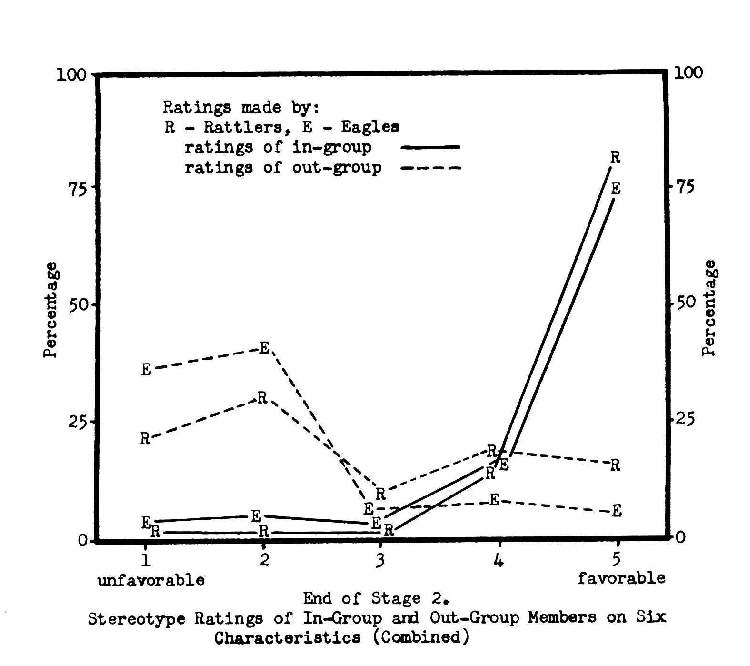
\includegraphics[width=0.49\textwidth]{Bilder/phase-zwei-ratings.jpg}}
	    \subfigure[Hütte der Klapperschlangen nach dem Überfall der Adler.]
	    {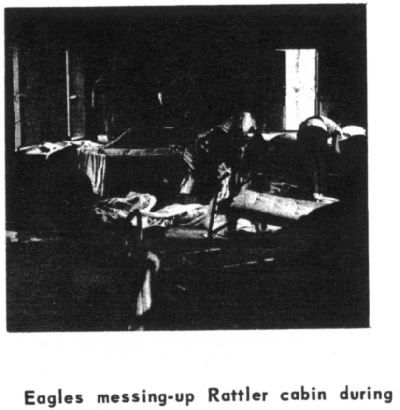
\includegraphics[width=0.38\textwidth]{Bilder/huette.jpg}}
		\caption{Resultat der zweiten Phase des Robbers-Cave-Experiments.}
	\label{fig:phase-zwei}
	\end{center}
\end{figure}

Beide Gruppen konnten Informationen austauschen und die Lücke an Wissen, die die Feindseligkeit zwischen den Lagern hervorrief, schließen. In einer abschließenden Befragung nach der dritten Phase des Experiments, gezeigt in Abbildung \ref{fig:phase-drei}, bewerteten sich beide Gruppen deutlich besser als noch eine Phase zuvor. \\

\begin{figure}[htbp]
	\begin{center}
		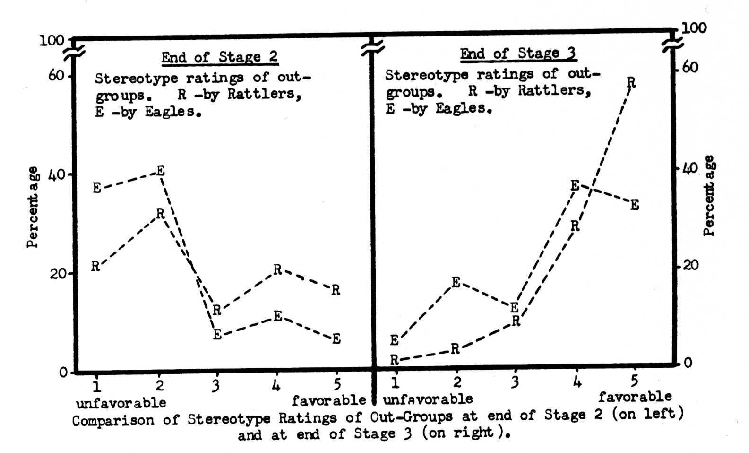
\includegraphics[width=0.6\textwidth]{Bilder/phase-drei-ratings.jpg}
		\caption{Die Bewertungen der beiden Gruppen nach der konfliktreichen Phase zwei (links) und der kooperativen Phase drei (rechts).}
		\label{fig:phase-drei}
	\end{center}
\end{figure}

Führungskräften zeigt das Robbers-Cave-Experiment, wie sich Menschen in Gruppen verhalten. Wenn es zu Konflikten innerhalb der Firma oder der Abteilung kommt, muss die Führungskraft in Erwägung ziehen, ob sich Gruppen gebildet haben, die in einem Konflikt stehen und so das Unternehmen wirtschaftlich beeinflussen. Stellt die Führungskraft fest, dass ein Gruppenkonflikt existiert, kann sie durch forcierte Kooperation zwischen den Gruppen den Konflikt lösen. \\

Das Robbers-Cave-Experiment zeigt ebenso die Notwendigkeit auf, innerbetrieblich Win-Win-Situationen herbeizuführen, wenn Konflikte vermieden werden sollen. Werden in einem Unternehmen Ressourcen verteilt, ist darauf zu achten, dass die im Verteilungsstreit unterlegene Partei nicht ohne neue Ressourcen aus der Aufteilung zurückkehrt. Ansonsten sind laut der Theorie des realistischen Gruppenkonflikts innerbetriebliche Konflikte sehr wahrscheinlich.

\subsubsection{Drang zu schnellem Handeln}
Wie in den letzten beiden Abschnitten gezeigt wurde, bremst uns das Überangebot an Informationen aus. Zeit, um Entscheidungen zu treffen, ist limitiert. Durch den nicht-abbrechenden Fluss an neuen Informationen müssen wir kontinuierlich Verarbeiten, um handlungsfähig zu bleiben. Dabei haben wir Mechanismen entwickelt, um die beiden Größen Zeit und Information in Einklang zu bringen. Diese führen jedoch zu Bias.

\begin{itemize}
	\item Wir haben das Gefühl, dass unser Handeln Einfluss hat auf Ereignisse, selbst, wenn dem nicht so ist. Wir neigen dazu, uns zu überschätzen. \cite{KRU99}
	\item Wir bevorzugen zeitnahe, vertraute Lösungen in räumlicher Näher vor Verzögertem und weit Entferntem. \cite{GRU15}
	\item Wir sind besonders motiviert, Dinge zu beenden, die wir bereits angefangen haben.\cite{MOO01}
	\item Wir sind bestrebt, unsere Autonomie und unseren Status in einer Gruppe zu erhalten und unwiderrufliche Entscheidungen zu vermeiden. \cite{JOS94}
	\item Wir bevorzugen Optionen, die einfach erscheinen oder über die wir mehr Informatioen haben vor solchen, die komplex und widersprüchlich wirken.\cite{FRI88}
\end{itemize}

Der Dunning-Kruger-Effekt soll als Beispiel für einen Bias dienen, bei dem wir aufgrund von mangelhaften Informationen und mangelhafter Zeit unsere Fähigkeiten überschätzen. Dunning und Kruger veröffentlichten 1999 gemeinsam ein Paper.\cite{KRU99} Das Paper beginnt mit der Geschichte des Bankräubers Wheeler, der im Jahr 1995 zwei Banken an ein- und demselben Tag überfiel. Besonders kurios an seiner Straftat war der Umstand, dass Wheeler vor der Tat sein Gesicht mit Zitronensaft besprenkelte. Das tat er in der Annahme, sein Gesicht würde für Dritte unsichtbar.\footnote{Der Catalogue of Bias, \href{https://catalogofbias.org/2018/03/22/twenty-years-of-bias-and-the-dunning-kruger-effect/}{abgerufen am 11.06.2018}.} Diese Eigenschaft schrieb er dem Fruchtsaft zu, da er um die Möglichkeit wusste, Zitronensaft als \glqq unsichtbare Tinte\grqq~zu verwenden. \\

Als die Polizei ihn unter Zuhilfenahme von Überwachungskameraufnahmen noch am selben Tag festnahm, soll er ausgerufen haben \glqq Aber ich hatte Saft aufgetragen!\grqq\footnote{Entnommen eines Blogs der \href{https://opinionator.blogs.nytimes.com/2010/06/20/the-anosognosics-dilemma-1/?_r=0}{New York Times}.} Nun könnte man diese Anekdote auf sich beruhen lassen und gegebenenfalls das US-amerikanische Bildungssystem kritisieren. Doch Dunning und Kruger nehmen sie zum Anlass für eine Untersuchung und finden schließlich ein System, das unter dem Namen \glqq Dunning-Kruger-Effekt\grqq~populärwissenschaftlichen Kultstatus erreicht hat. \\

\begin{figure}[htbp]
	\begin{center}
		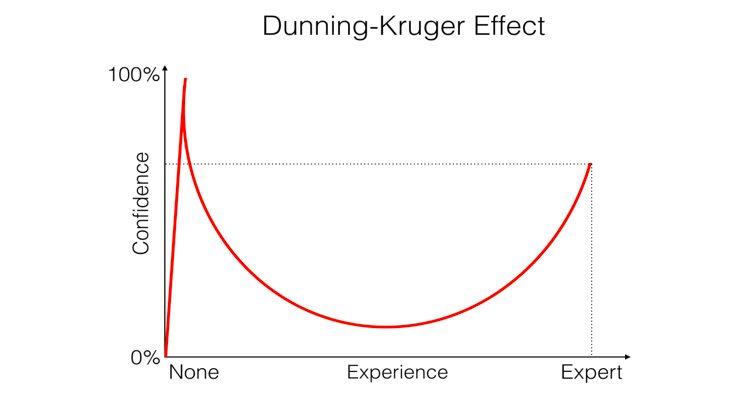
\includegraphics[width=0.95\textwidth]{Bilder/dunning-kruger.png}
		\caption{Die schematische Verdeutlichung des Dunning-Kruger-Effektes anhand eines Graphen. Grafik entnommen aus dem \glqq Catalogue of Bias\grqq~der University of Oxford.}
		\label{fig:dunning-kruger-effekt}
	\end{center}
\end{figure}

Ihre Untersuchungen mit Studenten zeigen, dass es ein Minimum an Erfahrung in einem Gebiet braucht, um die eigene Kompetenz korrekt einschätzen zu können. Unerfahrene überschätzen ihre eigenen Fähigkeiten in der Regel stark. Zu beachten ist, dass der Dunning-Kruger-Effekt nicht mit der Intelligenz einer Person korreliert. Auch ein sehr intelligenter Mensch, der wenig Fußball spielt, kann sich für einen guten Fußballer halten und seine Fähigkeiten überschätzen. Geht man dem Dunning-Kruger-Effekt auf den Leim, so ist man in einem Gebiet tatsächlich so unerfahren, dass man gar nicht weiß, wie unerfahren man ist (vergl. Abbildung \ref{fig:dunning-kruger-effekt}). \\

Personal mit Führungsverantwortung kann den Dunning-Kruger-Effekt auf zweierlei Weise in Entscheidungsprozesse einfließen lassen. Einerseits hilft er dabei, die eigenen Kompetenzen realistisch einzuschätzen. Die Frage zur Einschätzung der eigenen Fähigkeiten auf einem Gebiet könnte lauten: \glqq Verstehe ich das Thema so gut, dass ich weiß, was ich nicht weiß?\grqq. Ähnliche Denkmuster helfen beim Abschätzen der Kompetenz von Mitarbeitern. Hat der Kollege ein Bewusstsein für Probleme im Projekt, mit dem er beauftragt werden soll? Ist dem nicht so und strahlt er trotzdem großes Selbstvertrauen aus, dann gibt es Grund für Zweifel an der Kompetenz des Mitarbeiters. Es ist möglich, dass er noch ganz am Anfang seiner Lernkurve steht. \\

Nützlich zur Überprüfung des Verständnisses eines Mitarbeiters kann es auch sein, dass sich die Führungskraft etwas erklären lässt. Die \glqq Wissens-Illusion\grqq~(engl. \glqq illusion of explanatory depth\grqq) lässt Menschen glauben, etwas erklären zu können, ohne, dass sie tatsächlich in der Lage sind, dies zu tun. \footnote{Vergl. \href{https://www.edge.org/response-detail/27117}{Artikel auf edge.org, abgerufen am 18.06.2018}}

\subsubsection{Was sollten wir uns merken?}
Unser Gehirn greift zur Entscheidungsfindung auf unsere Erfahrungen zurück. In bewussten und unbewussten Prozessen werden Erinnerungen abgerufen und verarbeitet. Derart neu entstandenes Wissen wird nun wieder als Erinnerung abgelegt oder vergessen. Doch welche Eindrücke, welche Informationen merken wir uns? Tatsächlich haben Forscher Muster darin erkannt, was wir uns merken und was nicht.

\begin{itemize}
	\item Wir verändern und verstärken Erinnerungen, nachdem wir sie gespeichert haben. \cite{BRO91}
	\item Wir vergessen Details, um Verallgemeinerungen zu treffen. \cite{BAU01}
	\item Wir reduzieren Ereignisse und Listen auf ihre Kernelemente. \cite{KAH93}
	\item Wir speichern Erinnerungen abhängig davon, wie wir sie erleben.\cite{RHO00}
\end{itemize}

Die Kommunikationstheorie impliziert, dass zwei Personen die selbe Aussage grundsätzlich verschieden auffassen können.\footnote{Vergl. \href{https://www.schulz-von-thun.de/die-modelle/das-kommunikationsquadrat}{Schulz von Thun}} Rhodes und Anastasi gehen in ihrem Paper \glqq The effects of levels-of-processing manipulation on false recall\grqq\cite{RHO00} auf einen ähnlichen Effekt ein, indem sie zeigen, dass der Inhalt unserer Erinnerungen abhängig von den Umständen ist, unter denen wir sie aufgenommen haben. \\

Dazu bereiteten die beiden Forscher einen Versuch vor, in dem sie Wortlisten analysieren ließen. Diese Wortlisten beinhalten Begriffe, die zu einem anderen, übergeordneten Begriff gehören. Dieser übergenordnete Begriff, der sogenannte \glqq critical lure\grqq, ist jedoch selbst nicht in der Liste enthalten. Ein Beispiel wären die Liste der Begriffe \glqq spitz, Stich, krank, Arzt, Flüssigkeit\grqq, der dazugehörige critical lure ist \glqq Spritze\grqq. Der amerikanische Psychologe James Deese prägte den Begriff des \glqq critical lure\grqq~1959.\cite{DEE59} Er zeigte, dass aufmerksame Personen, denen eine Liste zu einem critical lure gezeigt wird, sich im Nachhinein an den critical lure erinnern können. \\

Rhodes und Anastasi orientierten sich in ihrem Vorgehen an Deese\cite{DEE59}, änderten den Versuch aber ab. Sie unterteilten die Versuchsteilnehmen in zwei Gruppen. Diesen beiden Gruppen wurden die selben Listen zu critical lures gezeigt. Jedoch erhielten die beiden Gruppen unterschiedliche Arbeitsaufträge: \\

Die erste Gruppe wurde beauftragt, die Vokale in jedem Wort zu zählen und sich das Ergebnis nach jedem Wort zu notieren. Der Gruppe wird ein flaches Niveau an kognitiver Anforderung gestellt, die Gruppe wird als \glqq Flach\grqq~bezeichnet. \cite[S.160]{RHO00} Die zweite Gruppe sollte den Grad der Abstraktheit eines jeden Begriffes auf einer Skala zwischen 1 und 5 bewerten. So ist \glqq Freiheit\grqq~als sehr abstrakter Begriff etwa mit einer 4 oder 5 zu bewerten. Hingegen wäre der Begriff \glqq Baum\grqq~mit einer 1 zu bewerten. Anschließend wurden beide Gruppen daraufhin getestet, an wieviele Begriffe aus den Listen sie sich erinnerten und an wie viele critical lures sie sich erinnerten.\\

Die Ergebnisse des Versuchs sind in Tabelle \ref{tab:memory} gezeigt. Die Versuchsgruppe, deren Mitglieder einen flachen Grad an kognitiver Interaktion mit den Begriffen der Liste hatte, schnitt deutlich schlechter ab als die Gruppe mit tiefer kognitiver Interaktion. So erinnerte sich die Gruppe mit tiefer Interaktion an 61\% mehr Begriffe aus den Listen. Zusätzlich konnten die Versuchsteilnehmer mit flacher kognitiver Anforderung nur halb so viele critical lures identifizieren, wie Teilnehmer aus der anderen Gruppe. \\

\begin{table}[htbp]
\begin{center}
\begin{tabular}{|c|c|c|}
\hline
Verarbeitungsebene & Anteil erinnerter Listenelemente & Anteil erinnerter Critical Lures \\ \hline
Flach & 18 \% & 23 \% \\ \hline
Tief & 29 \% & 47 \% \\ \hline
\end{tabular}
\end{center}
\caption{Ergebnis des Erinnerungsexperiments von Rhodes und Anastasi. Die beiden Versuchsgruppen sind nach dem Grad der kognitiven Anforderung in \glqq Flach\grqq~und \glqq Tief\grqq\ eingeteilt.}
\label{tab:memory}
\end{table}

Was Rhodes und Anastasi gezeigt haben ist somit, weshalb es von äußerster Wichtigkeit ist, dass Entscheidungen und Besprechungen verschriftlicht werden. Es ist nicht nur so, dass wir Vieles wieder vergessen, womit wir uns auseinandergesetzt haben. Vielmehr erinnern wir uns abhängig von unserer Beschäftigung. Jemand, der eine Besprechung leitet, wird sich anders and Inhalte erinnern als jemand, der in der selben Besprechung zu einem Thema referiert hat. Eine gemeinsame Erinnerung in Form eines Schriftstücks zu schaffen ist somit unabdingbar, um Zusammenarbeit überhaupt erst zu ermöglichen. \\

Dem voraus geht die Einsicht, dass man sich an Manches nicht erinnern kann - Führungskräfte sollten nicht versuchen abzustreiten, wenn sie sich irren, sondern einen Irrtum grundsätzlich als Möglichkeit betrachten. Besonders wichtig wird dies in Situationen, denen die Führungskraft eine andere Bedeutung zuordnet als der geführte Mitarbeiter. Wird in einem Gespräch beiläufig eine mögliche zukünftige Beförderung des Mitarbeiters erwähnt, hat dies eine große Bedeutung für den Mitarbeiter, der gegebenenfalls eine Erwartungshaltung entwickelt. Vergisst die Führungskraft diese beiläufige Bemerkung, kann es die Arbeitsmoral des Mitarbeiters nachhaltig negativ beeinflussen - die gesprochenen Worte der Führungskraft werden auf Seiten des Mitarbeiter als Handlung aufgefasst. Hier ist es, wie bereits vorher beschrieben, wichtig, Besprochenes zu verschriftlichen und Themen nach ihrer Relevanz für andere hin zu überprüfen, bevor sie angesprochen werden.